\section{Neural networks}

\subsection{Multi-layer perceptron}

\begin{marginfigure}
    \centering
    \incfig{perceptron}
    \caption{Computation graph of a perceptron \citep{rosenblatt1958perceptron}, where $\sigma(x) = \mathbb{1}\{ x > 0 \}$.}
    \label{fig:perceptron}
\end{marginfigure}

\begin{marginfigure}
    \centering
    \incfig{xor-problem}
    \caption{XOR problem. As can be seen, the data is not linearly separable, and thus not solvable by the perceptron.}
    \label{fig:xor-problem}
\end{marginfigure}

\begin{marginfigure}
    \centering
    \incfig{mlp}
    \caption{Example multi-layer perceptron architecture.}
    \label{fig:mlp}
\end{marginfigure}

The original perceptron \citep{rosenblatt1958perceptron} was a single layer perceptron with the
following non-linearity, \[
    \sigma(x) \doteq \mathbb{1}\{ x > 0 \}.
\]
The classification of a single point can then be written as \[
    \hat{y} = \mathbb{1}\{\transpose{\vec{w}}\vec{x} + b > 0\}.
\]
The learning algorithm then iteratively updates the weights for a data point that was classified
incorrectly, \[
    \vec{\theta} \gets \vec{\theta} + \eta \underbrace{(y_i - \hat{y}_i)}_{\text{residual}} \vec{x}_i,
\]
where $\eta$ is the learning rate. This is essentially gradient descent with a Hinge loss, where if
$y < \hat{y}$, then we decrease the weights, while if $y > \hat{y}$, we increase the weights. If
the data is linearly separable, the perceptron converges in finite time.

The problem with the single-layer perceptron was that it could not solve the XOR problem; see
\Cref{fig:xor-problem}. This can be solved by introducing hidden layers, \[
    \hat{y} = \sigma(\mat{W}_k \sigma(\mat{W}_{k-1} \cdots \sigma(\mat{W}_1 \vec{x}))).
\]
We call this architecture a multi-layer perceptron (MLP); see \Cref{fig:mlp}. We then want to
estimate the parameters $\vec{\theta} = \{ \mat{W}_1,\ldots,\mat{W}_k,\vec{b}_1,\ldots,\vec{b}_k
    \}$, using an optimization algorithm such as gradient descent, which we call ``learning``. We can
compute the gradient by backpropagation, which we will see in a later section.

\subsection{Loss functions}

We need an objective to optimize for. We typically call this objective function the loss function,
which we minimize. In classification, we typically optimize the \textit{maximum likelihood
    estimate} (MLE),
\begin{align*}
    \argmax_{\vec{\theta}} p(\mathcal{D}\mid \vec{\theta}) & \overset{\mathrm{iid}}{=} \argmax_{\vec{\theta}} \prod_{i=1}^n p(y_i \mid \vec{\theta})              \\
                                                           & = \argmin_{\vec{\theta}} -\log \prod_{i=1}^n p(y_i\mid\vec{\theta}) \margintag{$\log$ is monotonic.} \\
                                                           & = \argmin_{\vec{\theta}} -\sum_{i=1}^n \log p(y_i\mid\vec{\theta}).
\end{align*}
If the model predicts the parameters of a Bernoulli distribution,\sidenote{\Ie, $y \in \{ 0,1 \}$,
    but it predicts the probability of $y = 1$ with $\hat{y} \in [0,1]$.} MLE is equivalent to binary
cross-entropy,
\begin{align*}
    \mathcal{L}(\vec{\theta}) & = - \sum_{i=1}^{n} \log \mathrm{Ber}(y_i \mid \hat{y}_i \doteq f(\vec{x}_i\mid\vec{\theta})) \margintag{$f$ is a model that outputs the Bernoulli parameter. Note that this parameter must be in $[0,1]$, thus we use a sigmoid non-linearity, \[ \sigma(x) = \frac{1}{1 + \exp(-x)}. \]} \\
                              & = - \sum_{i=1}^{n} \log \hat{y}_i^{y_i} (1-\hat{y}_i)^{1-y_i}                                                                                                                                                                                                                             \\
                              & = - \sum_{i=1}^{n} y_i \log \hat{y}_i - (1-y_i) \log (1-\hat{y}_i).
\end{align*}
This loss is minimized if $y_i = \hat{y}_i$ for all $i \in [n]$; see \Cref{fig:bce-loss}. We can
extend this to multi-class classification by using the softmax and a categorical distribution.

\begin{marginfigure}[5cm]
    \centering
    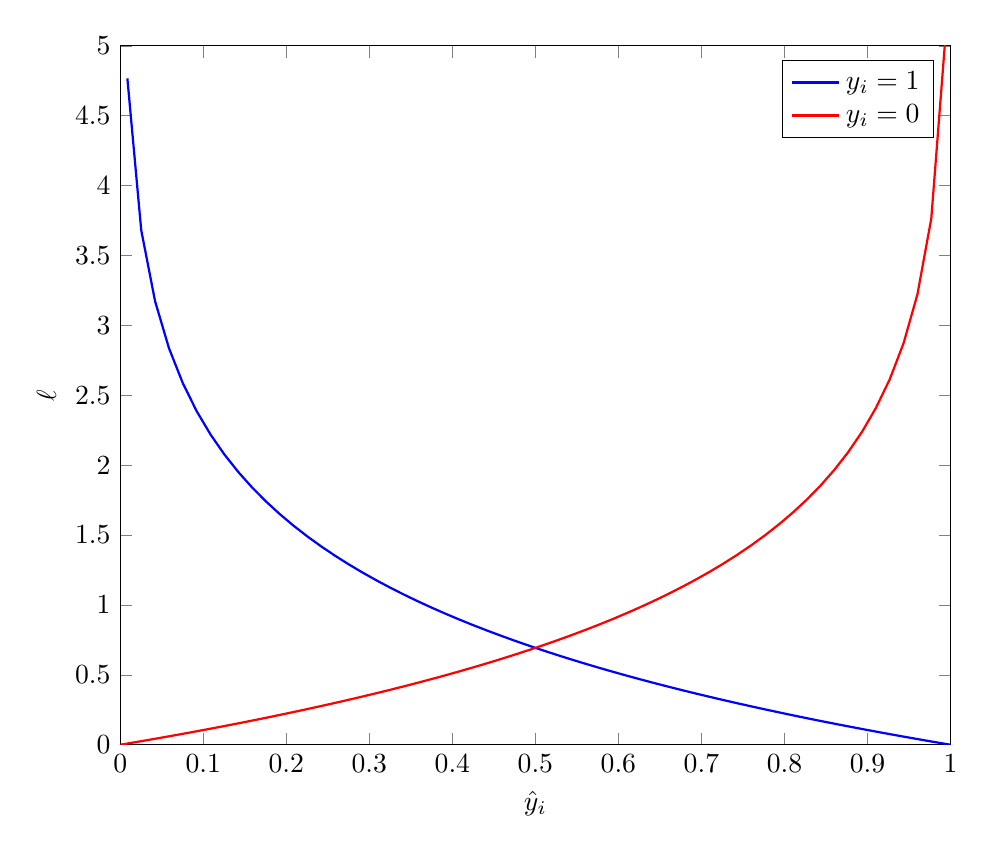
\begin{tikzpicture}
        \begin{axis}[
                xlabel={$\hat{y}_i$},
                ylabel={$\ell$},
                samples=600,
                xmin=0,
                xmax=1,
                ymin=0,
                ymax=5,
                width=\textwidth,
            ]
            \addplot [mark=none,color=blue,thick] {-ln(x)};
            \addlegendentry{$y_i = 1$};
            \addplot [mark=none, color=red,thick] {-ln(1-x)};
            \addlegendentry{$y_i = 0$};
        \end{axis}
    \end{tikzpicture}
    \caption{Loss function for if $y_i = 0$ and $y_i = 1$ in binary cross entropy.}
    \label{fig:bce-loss}
\end{marginfigure}

If we the choose the model to be Gaussian, we end up minimizing the mean-squared error, \[
    \mathcal{L}(\vec{\theta}) = \sum_{i=1}^{n} \| \vec{y}_i - f_{\vec{\theta}}(\vec{x}_i) \|_2^2.
\]
Furthermore, the Laplacian distribution yields minimizing the $\ell_1$ norm, \[
    \mathcal{L}(\vec{\theta}) = \sum_{i=1}^{n} \| \vec{y}_i - f_{\vec{\theta}}(\vec{x}_i) \|_1.
\]

If we have prior information about the weights $p(\vec{\theta})$, we could also optimize for the
\textit{maximum a posteriori} (MAP),
\begin{align*}
    \argmax_{\vec{\theta}} p(\vec{\theta}\mid \mathcal{D}) & = \argmax_{\vec{\theta}} p(\vec{\theta}) p(\mathcal{D}\mid\vec{\theta})                                               \\
                                                           & \overset{\mathrm{iid}}{=} \argmax_{\vec{\theta}} p(\vec{\theta}) \prod_{i=1}^n p(y_i\mid\vec{\theta}) p(\vec{\theta}) \\
                                                           & = \argmin_{\vec{\theta}} -\log \lft( p(\vec{\theta}) \prod_{i=1}^n p(y_i\mid\vec{\theta}) \rgt)                       \\
                                                           & = \argmin_{\vec{\theta}} - \log p(\vec{\theta}) - \sum_{i=1}^{n} \log p(y_i\mid \vec{\theta})                         \\
\end{align*}
Note that MAP and MLE are equivalent if $p(\vec{\theta})$ is uniform over the domain of weights.
Assuming a Gaussian prior distribution over $\vec{\theta}$, MAP yields Ridge regression, \[
    \mathcal{L}'(\vec{\theta}) = \mathcal{L}(\vec{\theta}) + \lambda \| \vec{\theta} \|_2^2.
\]

\subsection{Backpropagation}

Typically, we cannot find the optimal parameters $\vec{\theta}^\star$ in closed form, so we must
use an optimization algorithm. Optimization algorithms, such as gradient descent, typically require
computing the gradient \wrt the parameters. Backpropagation is an algorithm for computing the
gradient of any function, given that we have access to the derivatives of the primitive functions
it consists of.\sidenote{For example, to compute the gradient of $f(\vec{x},\vec{y}) =
        \sigma(\transpose{\vec{x}}\vec{y})$, we would need access to $\odv*{\sigma(x)}{x}$,
    $\pdv*{\transpose{\vec{x}}\vec{y}}{\vec{x}}$, and $\pdv*{\transpose{\vec{x}}\vec{y}}{\vec{y}}$.} It
then computes the gradient by making use of dynamic programming, the chain rule, and sum rule.

Let $\hat{y}_i < y_i$, then we want to increase $\hat{y}_i$ to match $y_i$. Furthermore, consider
the following loss function, \[
    \ell = \frac{1}{2} \lft( y - \hat{y} \rgt)^2, \quad \hat{y} = \sigma(\transpose{\vec{w}} \vec{h}),
\]
and the MLP architecture, then intuitively, we can do two things to increase $\hat{y}_i$:
\begin{enumerate}
    \item We could increase the weight connected to a node with a high activation value in the previous
          hidden layer. Typically, we optimize by moving the weights in the direction of the gradient, \[
              \pdv{\mathcal{L}}{w_k} = \pdv{\mathcal{L}}{\hat{y}} \pdv{\hat{y}}{\transpose{\vec{w}} \vec{h}} \pdv{\transpose{\vec{w}} \vec{h}}{w_k} = (y - \hat{y}) \sigma'\lft(\transpose{\vec{w}} \vec{h} \rgt) h_k.
          \]
          This matches our intuition, because the amount that we increase $w_k$ by is proportional to the
          activation connected to that weight $h_k$;

    \item Or, we could increase the activation that is connected to a strong weight in the previous hidden
          layer. Again, we move the weights in the direction of the gradient, \[
              \pdv{\mathcal{L}}{h_k} = \pdv{\mathcal{L}}{\hat{y}} \pdv{\hat{y}}{\transpose{\vec{w}} \vec{h}} \pdv{\transpose{\vec{w}} \vec{h}}{h_k} = (y - \hat{y}) \sigma' \lft( \transpose{\vec{w}} \vec{h} \rgt) w_k.
          \]
          This also matches our intuition, since the amount that we want to increase $h_k$ by is proportional
          to $w_k$. But, we cannot increase $h_k$ directly, but we can update the weights connected to $h_k$,
          which brings us back to the first case. This update will be proportional to
          $\pdv{\mathcal{L}}{h_k}$ by the chain rule. In this way, we can recursively update all the weights
          using gradient information.

\end{enumerate}

Thus, using first-order methods that iteratively move the weights in the direction of the gradient
should work well. Gradient descent iteratively updates the parameters by the following, \[
    \vec{\theta} \gets \vec{\theta} - \eta \grad{\mathcal{L}(\hat{\vec{y}},\vec{y})}{\vec{\theta}},
\]
until the gradient is small.

\subsection{Activation functions}

In MLPs, the activation function should be non-linear, or the resulting MLP is just an affine
mapping with extra steps. This is because the product of affine mappings are themselves affine
mappings.

\subsection{Universal approximation theorem}

\begin{theorem}[Universal approximation theorem \citep{hornik1989multilayer}]
    Let $\sigma: \R\to \R$ be a non-constant, bounded, and continuous activation function.
    Let $I_m$ denote the $m$-dimensional unit hypercube $[0,1]^m$ and the space of real-valued
    function on $I_m$ is denoted by $\mathcal{C}(I_m)$.

    Let $g \in \mathcal{C}(I_m)$ be any function in the hypercube. Let $\epsilon > 0, n\in \mathbb{N},
        v_i,b_i \in \R, \vec{w}_i \in \R^m$ for $i \in [n]$, then \[
        g(\vec{x}) \approx f_{\vec{\theta}}(\vec{x}) = \sum_{i=1}^{n} v_i \sigma(\transpose{\vec{w}_i} \vec{x} + b_i),
    \]
    where $|f_{\vec{\theta}}(\vec{x}) - g(\vec{x})| < \epsilon$ for all $\vec{x}\in I_m$.
\end{theorem}

The universal approximation theorem holds for any single hidden layer network. However, this hidden
layer may need to have infinite width to approximate $f$. In practice, deeper networks work better
than wider networks.
